\documentclass[a4paper,10pt,twoside]{article}
\usepackage[polish]{babel}
\usepackage[utf8]{inputenc}
\usepackage[T1]{fontenc}
\usepackage{indentfirst}
\usepackage[top=2.5cm, bottom=2.5cm, left=2.5cm, right=2.5cm]{geometry}
\usepackage{graphicx}
\usepackage{amsmath}
\usepackage{booktabs}

\begin{document}

\newcommand{\unit}[1]{\thinspace \mathrm{#1}}

\begin{center}
\bgroup
\def\arraystretch{1.5}
\begin{tabular}{|c|c|c|c|c|c|}
	\hline
	EAIiIB & \multicolumn{2}{|c|}{Piotr Morawiecki, Tymoteusz Paszun} & Rok II & {Grupa 3a} & {Zespół 6} \\
	\hline
	\multicolumn{3}{|c|}{\begin{tabular}{c}Temat: Moduł Younga \end{tabular}} &
	\multicolumn{3}{|c|}{\begin{tabular}{c}Numer ćwiczenia: 11 \end{tabular}} \\
	\hline
	\begin{tabular}{@{}c@{}}Data wykonania:\\8.11.2017r.\end{tabular} & \begin{tabular}{@{}c@{}}Data oddania:\\15.11.2017r.\end{tabular} &
	\begin{tabular}{c}Zwrot do poprawki:\\\phantom{data} \end{tabular} & \begin{tabular}{c}Data oddania:\\\phantom{data}\end{tabular} &
	\begin{tabular}{@{}c@{}}Data zaliczenia:\\\phantom{data}\end{tabular} & \begin{tabular}{c}Ocena:\\\phantom{ocena}\end{tabular} \\[4ex]
	\hline
\end{tabular}
\egroup
\end{center}


\section{Cel ćwiczenia}

Celem ćwiczenia jest wyznaczenie modułu Younga metodą statyczną przy pomocy pomiaru wydłużenia drutu wykonanego ze stali lub mosiądzu, obciążonego stałą siłą.

\section{Wstęp teoretyczny}

Prawo Hooke'a określa zależność odkształcenia od naprężenia. Według tego prawa odkształcenie ciała pod wpływem działającej na nie siły jest proporcjonalne do tej siły. Zależność ta pozostaje prawdziwa tylko dla niezbyt dużych odkształceń, nie przekraczających granicy Hooke'a, czyli maksymalnego naprężenia, przy którym zachodzące odkształcenie jest proporcjonalne do wywołującego je naprężenia. Odkształcenie opisane jest wzorem:
$$ \Delta l = \frac{Fl}{ES} $$

gdzie $ F $ - naprężenie, $ l $ - długość ciała, $ E $ - moduł Younga, $ S $ - pole przekroju poprzecznego ciała.

Moduł Younga ($E$) to współczynnik sprężystości podłużnej. Określa on własności sprężyste ciała stałego, charakteryzując podatność materiału na odkształcenia podłużne: rozciąganie, ściskanie, zgniatanie. Jego jednostką jest pascal ($\unit{Pa}$). Możemy go obliczyć znając naprężenie $\sigma$ występujące w danym obszarze ciała oraz względne odształcenie liniowe $\varepsilon$, co opisuje wzór:


$$ \sigma = E \varepsilon $$
gdzie:
$$ \varepsilon = \frac{\delta}{l}$$
$$\sigma = \frac{F}{S}$$
Wartość modułu Younga mówi nam jak duże naprężenie należaoby przyłożyć, aby zwiększyć dwukrotnie długość drutu. Taka zależność nie ma jednak odwzierciedlenia w praktyce, ponieważ już przy mniejszych naprężeniach ciało ulega nieodwracalnym zmianom.

Zgodnie z prawem Hooke'a zależność $\Delta l(F)$ jest liniowa, dlatego można ją opisać jako: $\Delta l(F)=aF+b$. Współczynnik kierunkowy to tangens kąta nachylenia prostej do osi OX, co opisujemy jako $a=\frac{\Delta l}{mg}$. Jest to równoznaczne z $a=\frac{l}{ES}$ (na podstawie Prawa Hooke'a), więc
$E=\frac{l}{aS}$. Podstawiając do równania $S=\frac{\pi d^2}{4}$ otrzymujemy wzór roboczy na moduł Younga:
$$E = \frac{4l}{\pi d^2 a}$$
Wartość współczynnika $a$ oraz jego niepewność $u(a)$ wyznaczymy korzystając z regresji liniowej.
\section{Wykonanie ćwiczenia}
\begin{enumerate}
	\item Zmierzenie długości drutu, który zostannie użyty w doświadczeniu, za pomocą przymiaru przymocowanego do statywu.
	\item Zamontowanie drutu w statywie i obciążenie szalki odważnikami, w celu naciągnięcia drutu. Pomiar średnicy drutu za pomocą śruby mikrometrycznej.
	\item Opróżnienie szlki z odważników, zwolnienie blokady belki pomiarowej. Regulacja naprężenia drutu, tak aby czujnik mikrometryczny został wyzerowany.
	\item Obciążanie szalki przez dokładanie kolejnych odważników, które zostały kolejno zważone. Notowanie w tabeli sumarycznej masy odważników i wydłużenia drutu. Dla lepszej dokładności pomiary zostały wykonane przy dokładaniu odważników i przy ich zdejmowaniu.
	\item Ponowne wykonanie poprzednich kroków dla drutu wykonanego z innego metalu.
\end{enumerate}

\begin{figure}[!htp]
\centerline{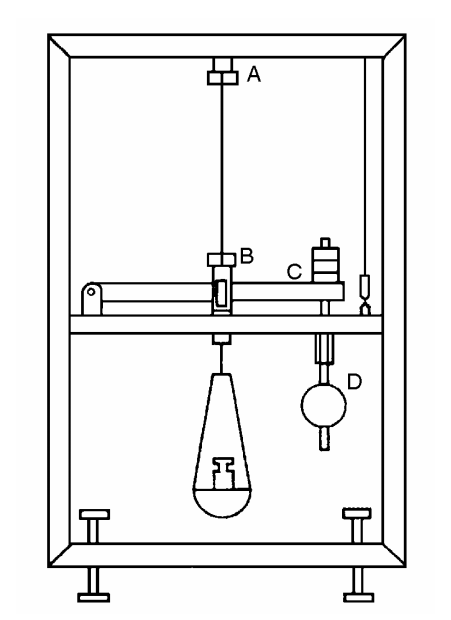
\includegraphics[scale=0.35]{przyrzad.png}}
\caption{Przyrząd pomiarowy}
\label{fig:tl}
\end{figure}

\newpage

\section{Wyniki pomiarów}

\subsection{Drut stalowy}

Zmierzona długość drutu: $ l = 1065 \unit{mm} $.
Średnica drutu: $ d = \frac{0,715 \unit{mm} + 0,705 \unit{mm} + 0,71 \unit{mm}}{3} = 0,71 \unit{mm}$.

\begin{table}[!htbp]
\caption{Pomiary wydłużenia dla drutu wykonanego ze stali}
\centering
\def\arraystretch{1.4}
\begin{tabular}{@{}rcccc@{}}
\\
\toprule
\begin{tabular}{@{}c@{}}Masa odważników $[\unit{kg}]$\end{tabular} &
\begin{tabular}{@{}c@{}}Siła $F \unit{[N]}$\end{tabular} &
\begin{tabular}{@{}c@{}}Wskazanie czujnika przy \\ dodawaniu obciążenia\end{tabular} &
\begin{tabular}{@{}c@{}}Wskazanie czujnika przy
\\ odejmowaniu obciążenia\end{tabular} &
\begin{tabular}{@{}c@{}}$\Delta l \unit{[mm]}$\end{tabular}\\
\midrule
0,957  &   9,38817  &  0,290  &  0,38  &  0,16750 \\
1,968  &  19,30608  &  0,780  &  0,83  &  0,40250 \\
2,956  &  28,99836  &  1,110  &  1,17  &  0,57000 \\
3,951  &  38,75931  &  1,425  &  1,48  &  0,72625 \\
4,918  &  48,24558  &  1,780  &  1,78  &  0,89000 \\
5,946  &  58,33026  &  2,070  &  2,07  &  1,03500 \\
6,928  &  67,96368  &  2,320  &  2,38  &  1,17500 \\
7,961  &  78,09741  &  2,630  &  2,65  &  1,32000 \\
8,989  &  88,18209  &  2,915  &  2,92  &  1,45875 \\
9,972  &  97,82532  &  3,230  &        &  1,61500 \\
\bottomrule
\end{tabular}
\end{table}

\subsection{Drut mosiężny}

Zmierzona długość drutu: $ l = 1070,5 \unit{mm} $.
Średnica drutu: $ d = \frac{0,79 \unit{mm} + 0,79 \unit{mm} + 0,795 \unit{mm}}{3} = 0,7917 \unit{mm}$.

\begin{table}[!htbp]
\caption{Pomiary wydłużenia dla drutu wykonanego z mosiądzu}
\centering
\def\arraystretch{1.4}
\begin{tabular}{@{}rcccc@{}}
\\
\toprule
\begin{tabular}{@{}c@{}}Masa odważników $[\unit{kg}]$\end{tabular} &
\begin{tabular}{@{}c@{}}Siła $F \unit{[N]}$\end{tabular} &
\begin{tabular}{@{}c@{}}Wskazanie czujnika przy \\ dodawaniu obciążenia\end{tabular} &
\begin{tabular}{@{}c@{}}Wskazanie czujnika przy
\\ odejmowaniu obciążenia\end{tabular} &
\begin{tabular}{@{}c@{}}$\Delta l \unit{[mm]}$\end{tabular}\\
\midrule
0,957  &   9,38817  &  0,42  &  0,43  &  0,2125  \\
1,968  &  19,30608  &  0,91  &  0,92  &  0,4575  \\
2,956  &  28,99836  &  1,31  &  1,33  &  0,6600  \\
3,951  &  38,75931  &  1,70  &  1,73  &  0,8575  \\
4,918  &  48,24558  &  2,06  &  2,08  &  1,0350  \\
5,946  &  58,33026  &  2,44  &        &  1,2200  \\
\bottomrule
\end{tabular}
\end{table}

\newpage

\section{Wykresy}

Na wykresach czerwonymi punktami oznaczone zostały uzyskane wyniki pomiarów. Niebieska linia to prosta regresji liniowej. Pomiar odstający od prostej regresji liniowej został oznaczony ciemniejszym okręgiem.

\begin{figure}[!htp]
\centerline{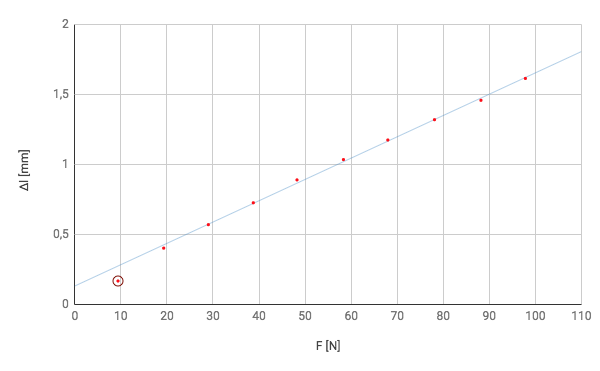
\includegraphics[scale=0.65]{steel_wire_first_point_marked.png}}
\caption{Wykres zależnosci wydłużenia drutu od przyłożonej siły dla stali}
\label{fig:tl}
\end{figure}

\begin{figure}[!htp]
\centerline{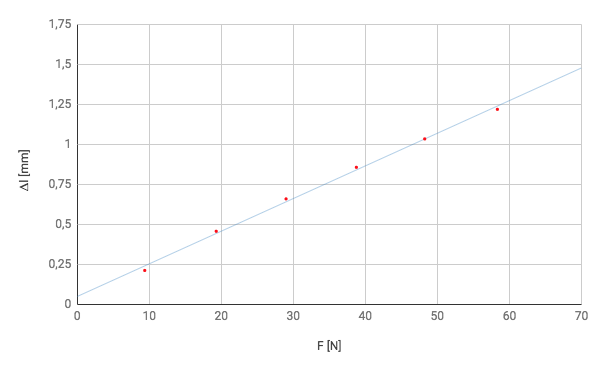
\includegraphics[scale=0.65]{brass_wire.png}}
\caption{Wykres zależnosci wydłużenia drutu od przyłożonej siły dla mosiądzu}
\label{fig:tl}
\end{figure}

\newpage

\section{Opracowanie wyników}

\subsection{Analiza błędów}

W wynikach pomiarów dla drutu stalowego zauważyliśmy odstawanie pierwszego punktu pomiarowego od prostej wyznaczonej metodą regresji liniowej. W dalszych obliczeniach odrzuciliśmy ten pomiar. Dla drutu wykonanego z mosiądzu nie zauważyliśmy odstawania żadnych punktów pomiarowych.

\subsection{Niepewności pomiarów}

Niepewność pomiaru długości drutu (typu B) - wynika z zastosowania przymiaru o podziałce o dokładności $ 1 \unit{mm} $:

$$ u(l) = \frac{1 \unit{mm}}{\sqrt{3}} = 0,577 \unit{mm} $$

Niepewność pomiaru wydłużenia drutu (typu B) wynika z zastosowania miernika mikrometrycznego o dokładności $ 1 \unit{mm} $:

$$ u(\Delta l) = \frac{0,01 \unit{mm}}{\sqrt{3}} = 0,00577 \unit{mm} $$

Niepewność pomiaru średnicy drutu (typu B) - wynika z zastosowania śruby mikrometrycznej o dokładności $ 0,01 \unit{mm} $:

$$ u(d) = \frac{0,01 \unit{mm}}{\sqrt{3}} = 0,00577 \unit{mm} $$

Niepewność wpółczynnika kierunkowego $ a = 1,523 \cdot 10^-5 \unit{\frac{m}{N}} $ dla prostej dopasowanej metodą najmniejszych kwadratów dla pomiarów drutu stalowego:

$$ u(a) = 4,275 \cdot 10^8 \unit{\frac{m}{N}} $$

Niepewność wpółczynnika kierunkowego $ a = 2,04 \cdot 10^-5 \unit{\frac{m}{N}} $ dla prostej dopasowanej metodą najmniejszych kwadratów dla pomiarów drutu wykonanego z mosiądzu:

$$ u(a) = 1,36 \cdot 10^7 \unit{\frac{m}{N}} $$

\subsection{Moduł Younga dla drutu stalowego}

Wartość modułu Younga:

$$ E = \frac{4l}{\pi d^2 a} = 176,61 \unit{GPa} $$

Niepewność złożona wyznaczonej wartości modułu Younga:

$$ \frac{u_c(E)}{E} = \sqrt{ \left( \frac{u(l)}{l} \right)^2 + \left( -2 \frac{u(d)}{d} \right)^2 + \left(-\frac{u(a)}{a} \right)^2} = \sqrt{ \left( \frac{0,577}{1065} \right)^2 + \left( -2 \frac{0,00577}{0,71} \right)^2 + \left( - \frac{4,275 \cdot 10^8}{0,00001582471518} \right)^2} = 0,016 $$


$$ u_c(E) =  E \cdot 0,016 = 2,826 \unit{[GPa]}$$

Niepewność rozszerzona:

$$ U(E) = k \cdot u_c(E) = 2 \cdot 2,826 \unit{[GPa]} = 5,652 \unit{[GPa]}$$


\subsection{Moduł Younga dla drutu z mosiądzu}

Wartość modułu Younga:

$$ E = \frac{4l}{\pi d^2 a} = 106,52 \unit{GPa} $$

Niepewność złożona wyznaczonej wartości modułu Younga:

$$ \frac{u_c(E)}{E} = \sqrt{ \left( \frac{u(l)}{l} \right)^2 + \left( -2 \frac{u(d)}{d} \right)^2 + \left(-\frac{u(a)}{a} \right)^2} = \sqrt{ \left( \frac{0,577}{1065} \right)^2 + \left( -2 \frac{0,00577}{0,71} \right)^2 + \left( - \frac{1,36 \cdot 10^7}{0,00002} \right)^2} = 0,0146 $$

$$ u_c(E) =  E \cdot 0,0146 = 1,556 \unit{[GPa]}$$

Niepewność rozszerzona:

$$ U(E) = k \cdot u_c(E) = 2 \cdot 1,556 \unit{[GPa]} = 3,112 \unit{[GPa]}$$

\subsection{Ocena zgodności uzyskanych wyników}

Różnica między obliczoną wartością modułu Younga dla stali ($ E = 176,61 \unit{GPa} $), a wartością tabelaryczną ($ E_0 = 200 \unit{GPa} $) wynosi:

$$ \vert E - E_0 \vert = \vert 176,61 \unit{GPa} - 200 \unit{GPa} \vert = 23,39 \unit{GPa} $$

Uzyskany wynik nie mieści się w niepewności rozszerzonej ($ U(E) = 5,652 \unit{[GPa]} $).


Różnica między obliczoną wartością modułu Younga dla mosiądzu ($ E = 106,52 \unit{GPa} $), a wartością tabelaryczną ($ E_0 = 100 \unit{GPa} $) wynosi:

$$ \vert E - E_0 \vert = \vert 106,52 \unit{GPa} - 100 \unit{GPa} \vert = 6,52 \unit{GPa} $$

Uzyskany wynik nie mieści się w niepewności rozszerzonej ($ U(E) = 3,112 \unit{[GPa]} $).


\section{Wnioski}

Określenie poprawności wyników doświadczeń jest trudne ze względu na duży rozrzut wartości tabelarycznych modułu Younga wg różnych źródeł. Wynika to z zależności modułu Younga od składu stopu danego materiału.

Wyliczony moduł Younga dla stali ($E = 176,61 \unit{GPa}$) znacznie odbiega od znalezionych wartości tabelarycznych ($E_0 = 190 - 220 \unit{GPa}$). Może być to spowodowane zużyciem badanego drutu.

Moduł Younga wyznaczony dla mosiądzu ($ E = 106,52 \unit{GPa} $) odbiega od wartości tabelarycznej podanej w opisie ćwiczenia, jednak mieści się w zakresie wartości tabelarycznych podanych w innych źródłach ($ E_0 = 103 - 124 \unit{GPa} $).

\end{document}
